\documentclass[10pt, a4paper]{jsarticle}
\usepackage[dvipdfm]{graphicx}
\usepackage{otf}
\usepackage{amsmath}
\usepackage{listings,jvlisting} %日本語のコメントアウトをする場合jvlisting(もしくはjlisting)が必要
%ここからソースコードの表示に関する設定
\lstset{
  basicstyle={\ttfamily},
  identifierstyle={\small},
  commentstyle={\smallitshape},
  keywordstyle={\small\bfseries},
  ndkeywordstyle={\small},
  stringstyle={\small\ttfamily},
  frame={tb},
  breaklines=true,
  columns=[l]{fullflexible},
  numbers=left,
  xrightmargin=0zw,
  xleftmargin=3zw,
  numberstyle={\scriptsize},
  stepnumber=1,
  numbersep=1zw,
  lineskip=-0.5ex,
  keepspaces=true,
}
\title{複雑系科学演習 第2回 レポート} % タイトルを決める作業
\begin{document} % 文書の始まり
\author{複雑系知能学科 複雑系コース 3年 Iクラス番号1019086 岩上慎之介}
\maketitle % 決めたタイトルを挿入する作業
\newpage
% \tableofcontents
\section{レポート課題 1st}

\subsection{課題1}
前頁の関数nextをテント写像に書き換え,リターンマップを描け\\
\subsubsection{画像}
\begin{figure}[htbp]
  \centering
  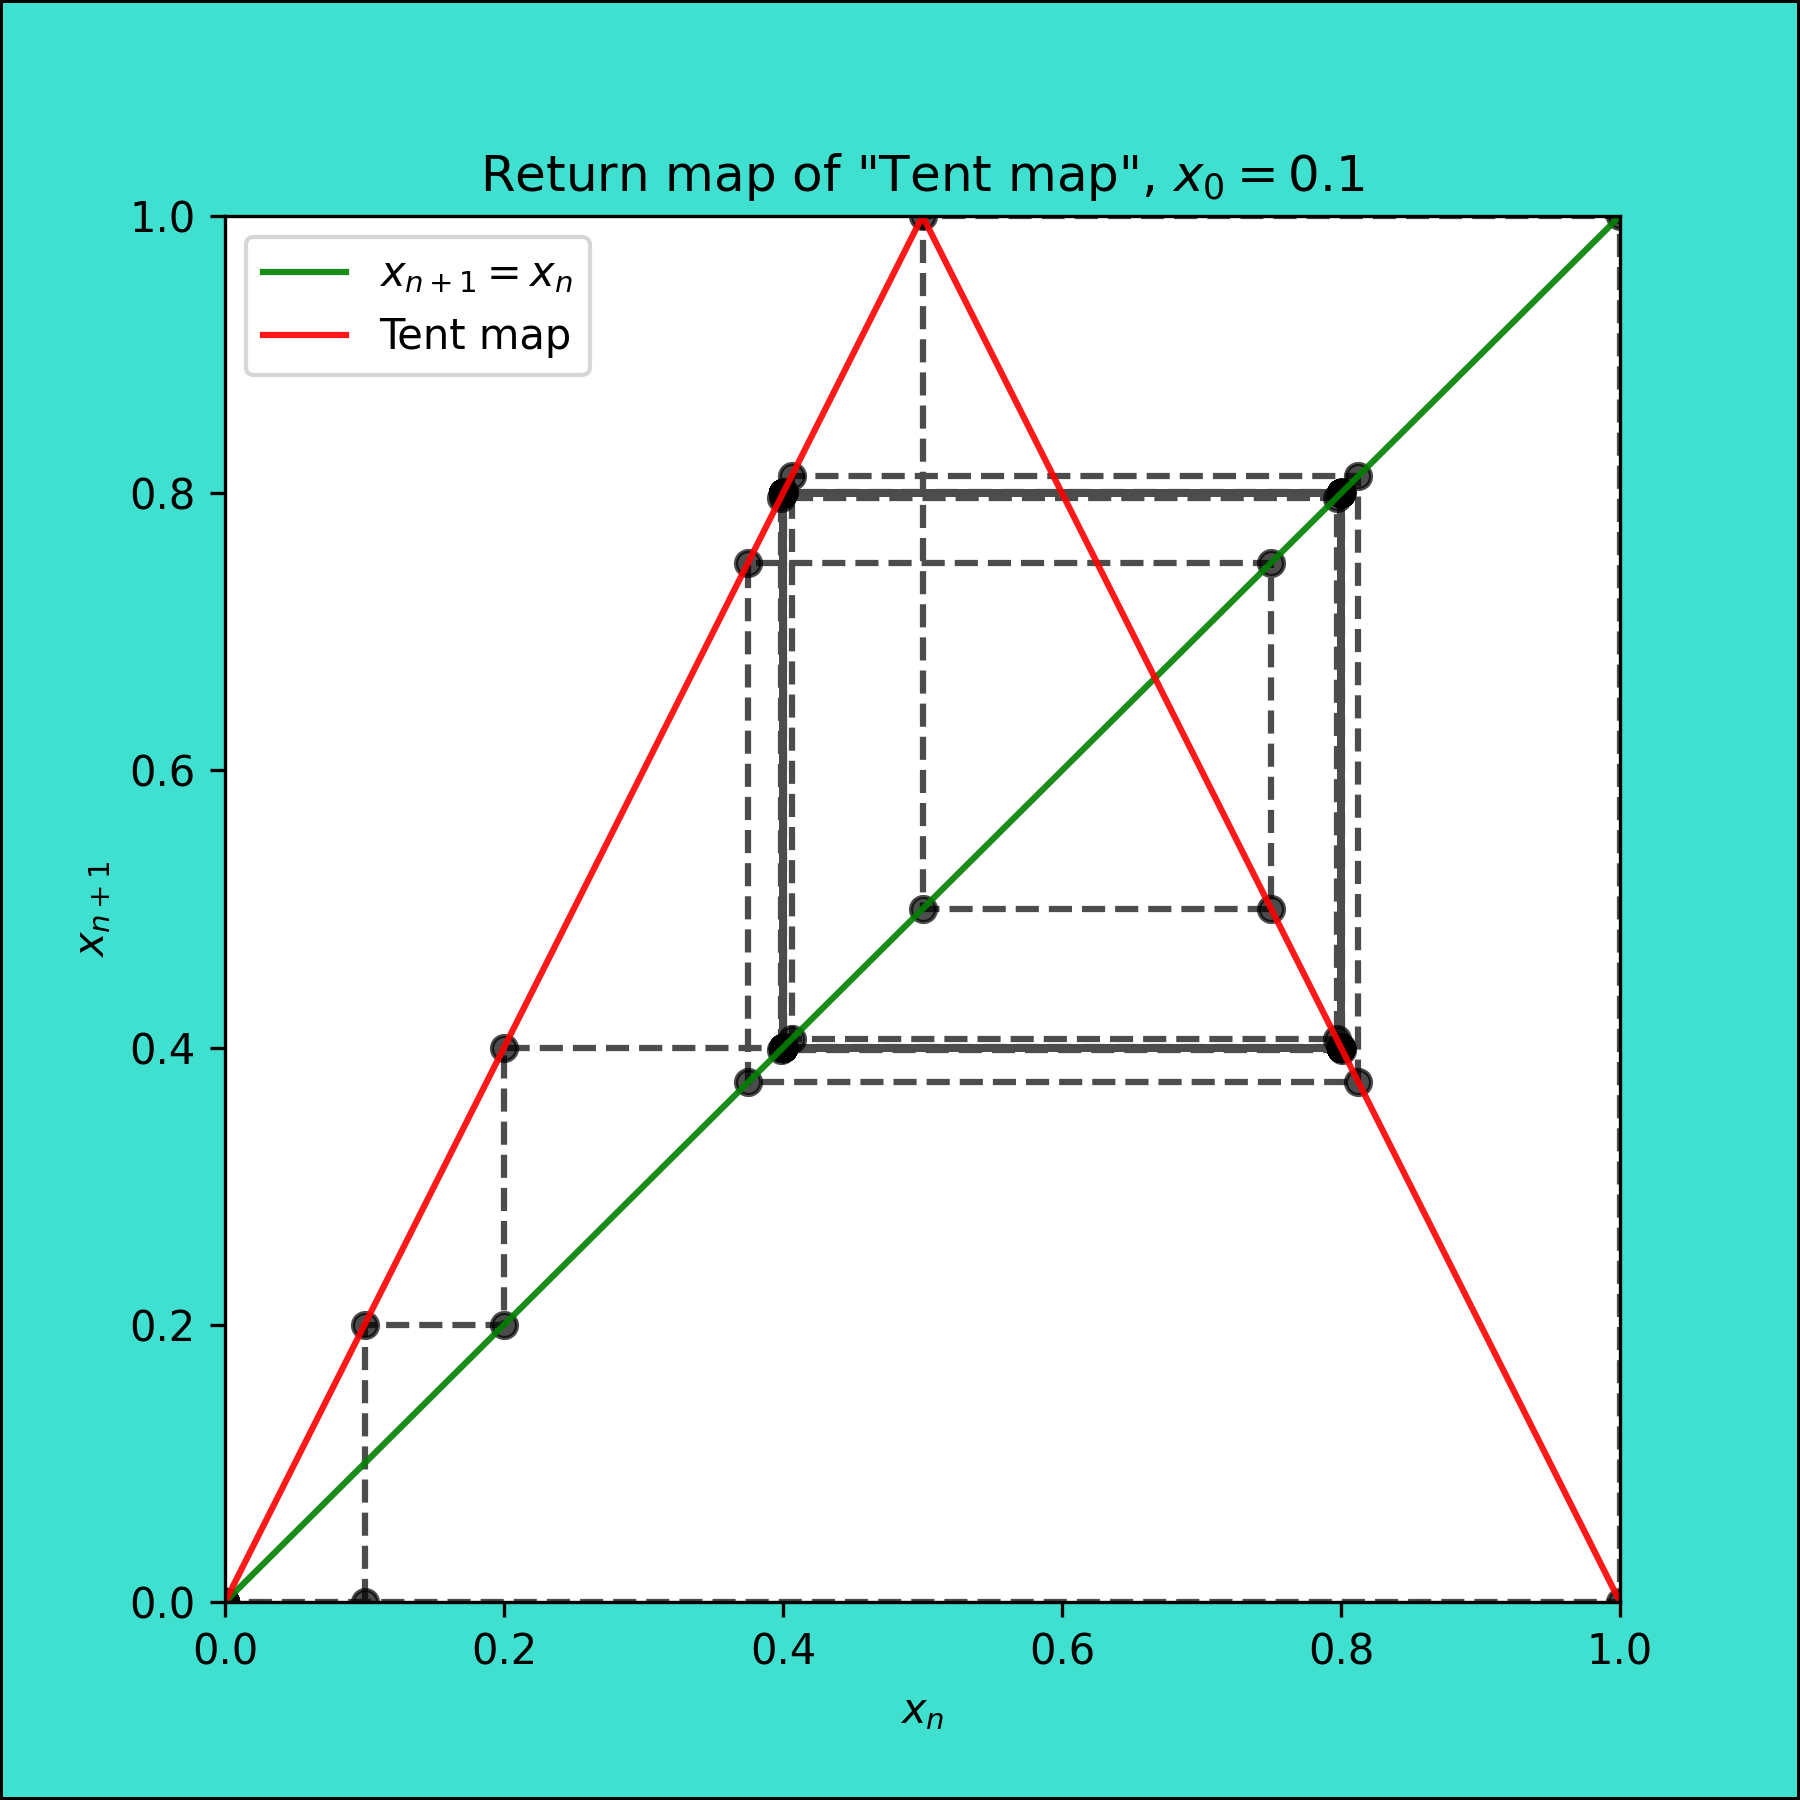
\includegraphics[keepaspectratio, scale=0.7]{images/Problem6/task6.png}
\end{figure}

\subsubsection{ソースコード}
\begin{lstlisting}[caption=task6]
  from matplotlib import pyplot as plt
  import numpy as np


  class Task6():
      def __init__(self) -> None:
          self.x = 0.1                      # 初期値 x0 = 0.1
          self.xn = np.linspace(0, 1, 1000)  # 横軸の範囲と刻み幅
          self.tent_y = []                  # テント写像のグラフを描くための配列
          for i in self.xn:
              if 0 <= i <= 0.5:
                  self.tent_y.append(2 * i)
              else:
                  self.tent_y.append(2 * (1 - i))
          self.filepath = '複雑系科学演習/Week6/images/task6'

      def tent(self) -> list:
          "リターンマップでのテント写像の座標を持つ配列を返す"
          calc_x = self.x
          x_array = [calc_x]
          for _ in range(100):
              if 0 <= calc_x <= 0.5:
                  calc_x = 2 * calc_x
              else:
                  calc_x = 2 * (1 - calc_x)
              x_array.append(calc_x)
          return x_array

      def plot_return_map(self) -> None:
          "リターンマップの描画(テント写像)"
          plt.figure(figsize=(6, 6), facecolor='turquoise',
                    linewidth=1, edgecolor='black')
          n = self.tent()
          spiper_plot_x = [self.x]          # クモの巣図用の配列(x)
          spiper_plot_y = [0]               # クモの巣図用の配列(y)
          for i in range(1, len(n)):
              spiper_plot_x.append(n[i - 1])
              spiper_plot_x.append(n[i])
              spiper_plot_y.append(n[i])
              spiper_plot_y.append(n[i])

          plt.plot(spiper_plot_x, spiper_plot_y, marker='o',
                  linestyle='dashed', color='black', alpha=0.7)
          plt.plot(self.xn, self.xn, color='green',
                  alpha=0.9, label="$x_{n+1} = x_n$")
          plt.plot(self.xn, self.tent_y, color='red',
                  alpha=0.9, label="Tent map")
          plt.title("Return map of \"Tent map\", $x_0 = $" + str(self.x))
          plt.xlim(0, 1)
          plt.ylim(0, 1)
          plt.xlabel("$x_n$")
          plt.ylabel("$x_{n+1}$")
          plt.legend(loc='best')
          plt.savefig(self.filepath, dpi=300)


  task = Task6()
  task.plot_return_map()
\end{lstlisting}


\subsection{課題2}
$x_0 = \dfrac{1}{10}$ として、どのような周期解になるか厳密にて計算せよ。\\\\
手計算で $x_i$ の値を計算すると、
\begin{equation}
  \begin{split}
    x_0& = \dfrac{1}{10}\\
    x_1& = 2 \times \dfrac{1}{10} = \dfrac{1}{5}\\
    x_2& = 2 \times \dfrac{1}{5} = \dfrac{2}{5}\\
    x_3& = 2 \times \dfrac{2}{5} = \dfrac{2}{5}\\
    x_4& = 2 \times \left( 1 - \dfrac{4}{5} \right) = \dfrac{2}{5}\\
    x_5& = 2 \times \dfrac{2}{5} = \dfrac{2}{5}\\
    x_6& = 2 \times \left( 1 - \dfrac{4}{5} \right) = \dfrac{2}{5}\\
    .\\.\\.
  \end{split}
\end{equation}
となるため $\dfrac{2}{5}$ と $\dfrac{4}{5}$ の2つの周期解(2周期解)を取り続けていく。

\subsection{課題3}
$x_0 = \dfrac{1}{10}$ として、前のプログラムを実行せよ。ただし $N = 100$ とし $x_{100}$ まで数値計算せよ。どのような結果となったか。理由も述べよ。

\subsubsection{出力}
\begin{lstlisting}[caption=out]
  0.700000 0.600000
  0.600000 0.600000
  0.600000 0.800000
  0.800000 0.800000
  0.800000 0.400000
  0.400000 0.400000
  0.400000 0.800000
  0.800000 0.800000
  0.800000 0.400000
  0.400000 0.400000
  0.400000 0.800000
  0.800000 0.800000
  0.800000 0.400000
  0.400000 0.400000
  0.400000 0.800000
  0.800000 0.800000
  0.800000 0.400000
  0.400000 0.400000
  0.400000 0.800000
  0.800000 0.800000
  0.800000 0.400000
  0.400000 0.400000
  0.400000 0.800000
  0.800000 0.800000
  0.800000 0.400000
  0.400000 0.400000
  0.400000 0.800000
  0.800000 0.800000
  0.800000 0.400000
  0.400000 0.400000
  0.400000 0.800000
  0.800000 0.800000
  0.800000 0.400000
  0.400000 0.400000
  0.400000 0.800000
  0.800000 0.800000
  0.800000 0.400000
  0.400000 0.400000
  0.400000 0.800000
  0.800000 0.800000
  0.800000 0.400000
  0.400000 0.400000
  0.400000 0.800000
  0.800000 0.800000
  0.800000 0.400000
  0.400000 0.400000
  0.400000 0.800000
  0.800000 0.800000
  0.800000 0.400000
  0.400000 0.400000
  0.400000 0.800000
  0.800000 0.800000
  0.800000 0.400000
  0.400000 0.400000
  0.400000 0.800000
  0.800000 0.800000
  0.800000 0.400000
  0.400000 0.400000
  0.400000 0.800000
  0.800000 0.800000
  0.800000 0.400000
  0.400000 0.400000
  0.400000 0.800000
  0.800000 0.800000
  0.800000 0.400000
  0.400000 0.400000
  0.400000 0.799999
  0.799999 0.799999
  0.799999 0.400002
  0.400002 0.400002
  0.400002 0.800003
  0.800003 0.800003
  0.800003 0.399994
  0.399994 0.399994
  0.399994 0.799988
  0.799988 0.799988
  0.799988 0.400024
  0.400024 0.400024
  0.400024 0.800049
  0.800049 0.800049
  0.800049 0.399902
  0.399902 0.399902
  0.399902 0.799805
  0.799805 0.799805
  0.799805 0.400391
  0.400391 0.400391
  0.400391 0.800781
  0.800781 0.800781
  0.800781 0.398438
  0.398438 0.398438
  0.398438 0.796875
  0.796875 0.796875
  0.796875 0.406250
  0.406250 0.406250
  0.406250 0.812500
  0.812500 0.812500
  0.812500 0.375000
  0.375000 0.375000
  0.375000 0.750000
  0.750000 0.750000
  0.750000 0.500000
  0.500000 0.500000
  0.500000 1.000000
  1.000000 1.000000
  1.000000 0.000000
  0.000000 0.000000
  0.000000 0.000000
  0.000000 0.000000
  0.000000 0.000000
  0.000000 0.000000
  0.000000 0.000000
  0.000000 0.000000
  0.000000 0.000000
  0.000000 0.000000
  0.000000 0.000000
  0.000000 0.000000
  0.000000 0.000000
  0.000000 0.000000
  0.000000 0.000000
  0.000000 0.000000
  0.000000 0.000000
  0.000000 0.000000
  0.000000 0.000000
  0.000000 0.000000
  0.000000 0.000000
  0.000000 0.000000
  0.000000 0.000000
  0.000000 0.000000
  0.000000 0.000000
  0.000000 0.000000
  0.000000 0.000000
  0.000000 0.000000
  0.000000 0.000000
  0.000000 0.000000
  0.000000 0.000000
  0.000000 0.000000
  0.000000 0.000000
  0.000000 0.000000
  0.000000 0.000000
  0.000000 0.000000
  0.000000 0.000000
  0.000000 0.000000
  0.000000 0.000000
  0.000000 0.000000
  0.000000 0.000000
  0.000000 0.000000
  0.000000 0.000000
  0.000000 0.000000
  0.000000 0.000000
  0.000000 0.000000
  0.000000 0.000000
  0.000000 0.000000
  0.000000 0.000000
  0.000000 0.000000
  0.000000 0.000000
  0.000000 0.000000
  0.000000 0.000000
  0.000000 0.000000
  0.000000 0.000000
  0.000000 0.000000
  0.000000 0.000000
  0.000000 0.000000
  0.000000 0.000000
  0.000000 0.000000
  0.000000 0.000000
  0.000000 0.000000
  0.000000 0.000000
  0.000000 0.000000
  0.000000 0.000000
  0.000000 0.000000
  0.000000 0.000000
  0.000000 0.000000
  0.000000 0.000000
  0.000000 0.000000
  0.000000 0.000000
  0.000000 0.000000
  0.000000 0.000000
  0.000000 0.000000
  0.000000 0.000000
  0.000000 0.000000
  0.000000 0.000000
  0.000000 0.000000
  0.000000 0.000000
  0.000000 0.000000
  0.000000 0.000000
  0.000000 0.000000
  0.000000 0.000000
  0.000000 0.000000
  0.000000 0.000000
  0.000000 0.000000
  0.000000 0.000000
  0.000000 0.000000
  0.000000 0.000000
  0.000000 0.000000
  0.000000 0.000000
  0.000000 0.000000
  0.000000 0.000000
  0.000000 0.000000
  0.000000 0.000000
  0.000000 0.000000
  0.000000 0.000000
  0.000000 0.000000
\end{lstlisting}

\subsubsection{結果と考察}
実行した結果、$0.4$ と $0.8$ でずっとループすることはなく途中から値が変化した。最終的には、$(x_n, x_{n+1}) = (0, 0)$ を取り続けるようになった。これは、コンピュータの丸め誤差が影響し値が変化したと考えられる。
\subsubsection{ソースコード}
\begin{lstlisting}[caption=tent.c]
  #include<stdio.h>
  #define N 100
  double next(double x, double r) {
      if (0 <= x && x <= 0.5) {
          return 2 * x;
      } else {
          return 2 * (1 - x);
      }
  }
  int main(void){
      int n;
      double r;
      double xn = 0.7;
      double xn1;
      scanf("%lf", &r);
      for(n = 0; n <= N; n++) {
          xn1 = next(xn, r);
          printf("%lf %lf\n", xn, xn1);
          printf("%lf %lf\n", xn1, xn1);
          xn = xn1;
      }
      return 0;
  }
\end{lstlisting}

\subsection{課題4}
テント写像のリアプノフ指数を計算せよ。プログラミングが必要なければ手計算でよい。\\
リアプノフ指数 $\lambda$ は、\\
\begin{equation}
  \lambda = \lim_{n \to \infty} \dfrac{1}{n} \sum_{i = 0}^{n-1} \log |f'(x_i)|
\end{equation}
と表すことができる。\\
今回はテント写像のリアプノフ指数について調べていくので、関数 $f(x_i)$ は、
\begin{equation}
  f(x_i) =
    \begin{cases}
      2x_i & \left( 0 \leq x_i \leq \dfrac{1}{2} \right)\\
      2(1 - x_i) & \left( \dfrac{1}{2} < x_i \leq 1 \right)
    \end{cases}
\end{equation}
となる。さらに $(3)$ を用いて計算すると $f'(x_i)$は、
\begin{equation}
  f'(x_i) =
    \begin{cases}
      2 & \left( 0 \leq x_i \leq \dfrac{1}{2} \right)\\
      -2 & \left( \dfrac{1}{2} < x_i \leq 1 \right)
    \end{cases}
\end{equation}
となる。よって、$|f'(x_i)| = 2$ である。したがって、テント写像のリアプノフ指数 $\lambda$ は、
\begin{equation}
  \begin{split}
    \lambda& = \lim_{n \to \infty} \dfrac{1}{n} \sum_{i = 0}^{n-1} \log 2\\
    & = \lim_{n \to \infty} \dfrac{1}{n} \times n \log 2\\
    & = \lim_{n \to \infty} \log 2\\
    & = \log 2
  \end{split}
\end{equation}
と計算することができ $\lambda = \log 2$ となる。 

\subsection{課題5}
テント写像は $x_n$ から $x_{n+1}$ を求める写像である。 $y_n = \sin^2 \left( \dfrac{\pi}{2} x_n \right)$ と定義して、 $y_{n+1}$ を $y_n$ の式として表わせ。\\
\end{document}